\parindent=0em
\section{Javier Cordero Calvo}
\noindent

La primera vez que interactué con la realidad extendida como desarrollador y no como usuario (previamente había probado la realidad virtual de \textit{Play Station}) fue algunas semanas antes de proponer el tema de este trabajo a mi compañero y al tutor. Para comprobar la viabilidad de un proyecto como este, comencé a investigar toda la tecnología hasta la fecha existente, tanto de realidad virtual, realidad aumentada y realidad mixta.\\

Una vez aprobado el tema del trabajo, comencé a realizar pequeños proyectos a modo de prueba con \textit{Vuforia}, pero debido a la falta de un dispositivo compatible con dicha tecnología, me fue imposible continuar con las pruebas. Sin embargo, decidí generar una aplicación de realidad aumentada sin aplicaciones XR de terceros. Para ello, dentro de Unity simplemente creé una cámara y una imagen de textura ligada a esta, de tal manera que siempre estuviese delante de la cámara. Una vez tenía estos elementos, probé a generar un objeto tridimensional dentro de la aplicación y así comprobar que si movía la cámara y el plano de textura por consiguiente, y el objeto se encontraba entre estos dos, se podría superponer a la realidad.\\

Una vez comprobado que esto funcionaba añadí el giróscopo y el acelerómetro del dispositivo a la fórmula del movimiento para así, si se movía tanto la cámara como el plano de textura y existía un objeto virtual en la escena, este se quedaría en su lugar de origen y no seguiría a la cámara en todo momento.\\

Finalmente, y dado que el trabajo a realizar contenía la idea de mezclar esta tecnología con mapas, creé un objeto a modo de brújula, que utilizaba la brújula del dispositivo para apuntar siempre al norte y situar esta con realidad aumentada dentro de la aplicación.\\

\begin{figure}[H]
    \centering
    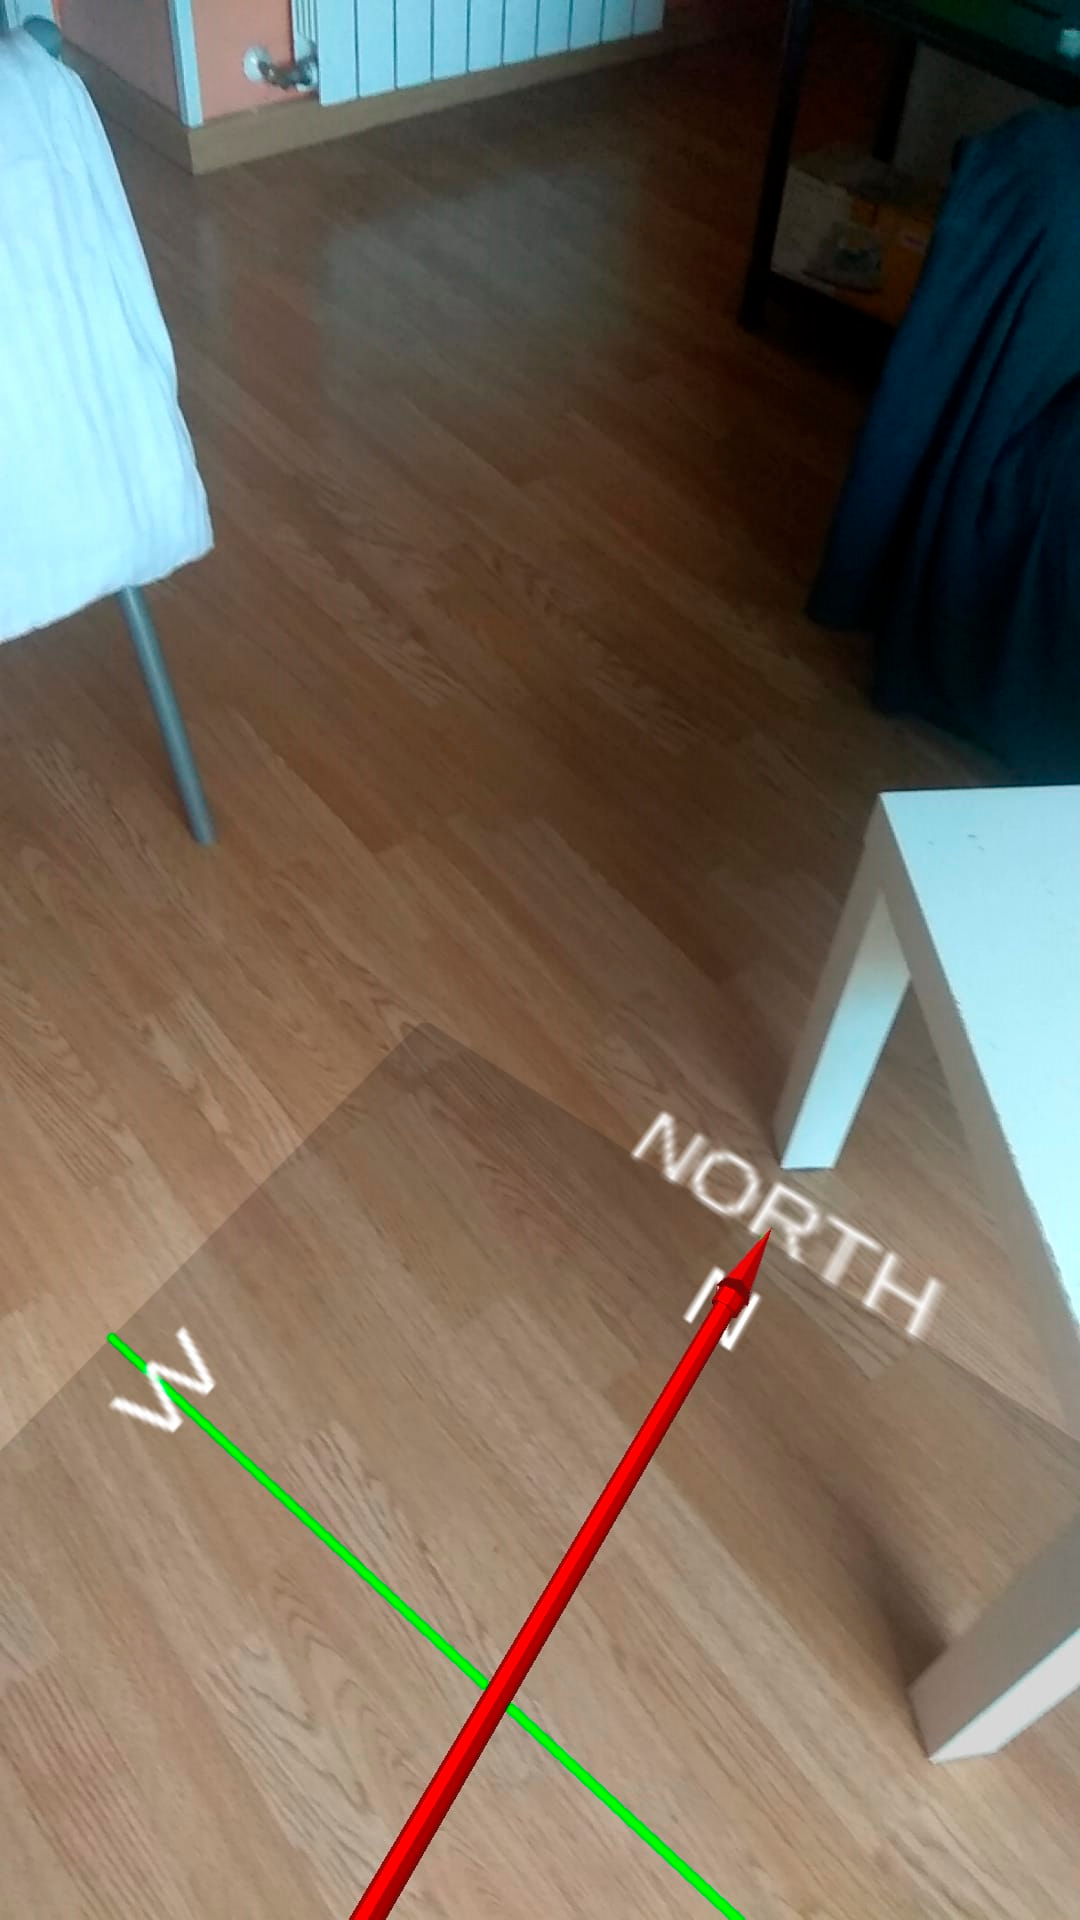
\includegraphics[scale=0.13]{Sections/Contribuciones/Imagenes/Brujula.png}
    \caption[Aplicación de brújula con realidad aumentada.]{Aplicación de brújula con realidad aumentada.}
    \label{fig:Brujula}
\end{figure}

Tras tener funcionando la aplicación de la brújula, y antes de comenzar el curso académico 2019/2020, también investigué la tecnología ofrecida por Mapbox para la geolocalización y generé una aplicación con las escenas de prueba que estos ofrecían en Unity. Esta aplicación sería usada en el futuro para facilitar la integración de ARCore con Mapbox.\\

Una vez dispusimos de los teléfonos móviles compatibles con ARCore, mi labor principal fue la de integrar esta tecnología con Unity y poder generar una aplicación que funcionase en el dispositivo. Para ello, dentro de Unity, investigué todos los paquetes que podrían servir de ayuda para o bien hacer que funcione o facilitar su uso. También investigué cuales eran los requisitos mínimos para la aplicación de ARCore que un móvil debía tener así como el tipo de renderizado con el que debía contar. Estas pruebas las realicé sobre uno de los ejemplos que incorpora ARCore, llamado \textit{HelloAR}.\\

El siguiente paso que realicé fue conocer en profundidad el funcionamiento de la API de ARCore dentro de Unity para poder modificarla en un futuro si fuese necesario. Para ello utilicé todos los scripts que encontré en la escena HelloAR y fui progresivamente entendiendo su funcionamiento y las acciones que realizaba para generar la nube de puntos.\\

Una vez comprendido el funcionamiento de esta, comencé a modificar varios factores que la misma aplicación ofrecía para obtener distintos resultados, como pueden ser el grosor de los puntos o el número de puntos que generaban. A su vez, dado que ARCore crea una nube de puntos con una malla, procedí a eliminarla y generar puntos propios para comprobar el funcionamiento sin malla.\\

Tras este punto y dado que ARCore me permitía únicamente una serie de acciones públicas a realizar en el editor, generé mi script propio para poder modificar todas las variables y factores que me conviniesen. Por lo tanto, copié el código de ARCore y lo lleve a una clase propia controlada por mí.\\

Dentro de esta ahora modifiqué todos los valores que tenía ARCore, cambiando por ejemplo las formas de objetos que instanciaba, eligiendo cuándo quería instanciarlos y cuando no. Para realizar las pruebas, instanciaba en cada uno de los \textit{ticks} de la aplicación un objeto para realizar la oclusión, aunque después este comportamiento debido a su baja eficiencia lo modifiqué, generando la \textit{Pool} de objetos de la nube de puntos para cualquier tamaño de esta.\\

Una vez tenía todos los puntos y podía modificar sus formas desde el editor, intenté mediante el Line Renderer proporcionado por Unity generar una oclusión mediante la unión de todos los puntos de la nube. Esta idea sin embargo, una vez realizada, fue totalmente descartada.\\

\begin{figure}[H]
    \centering
    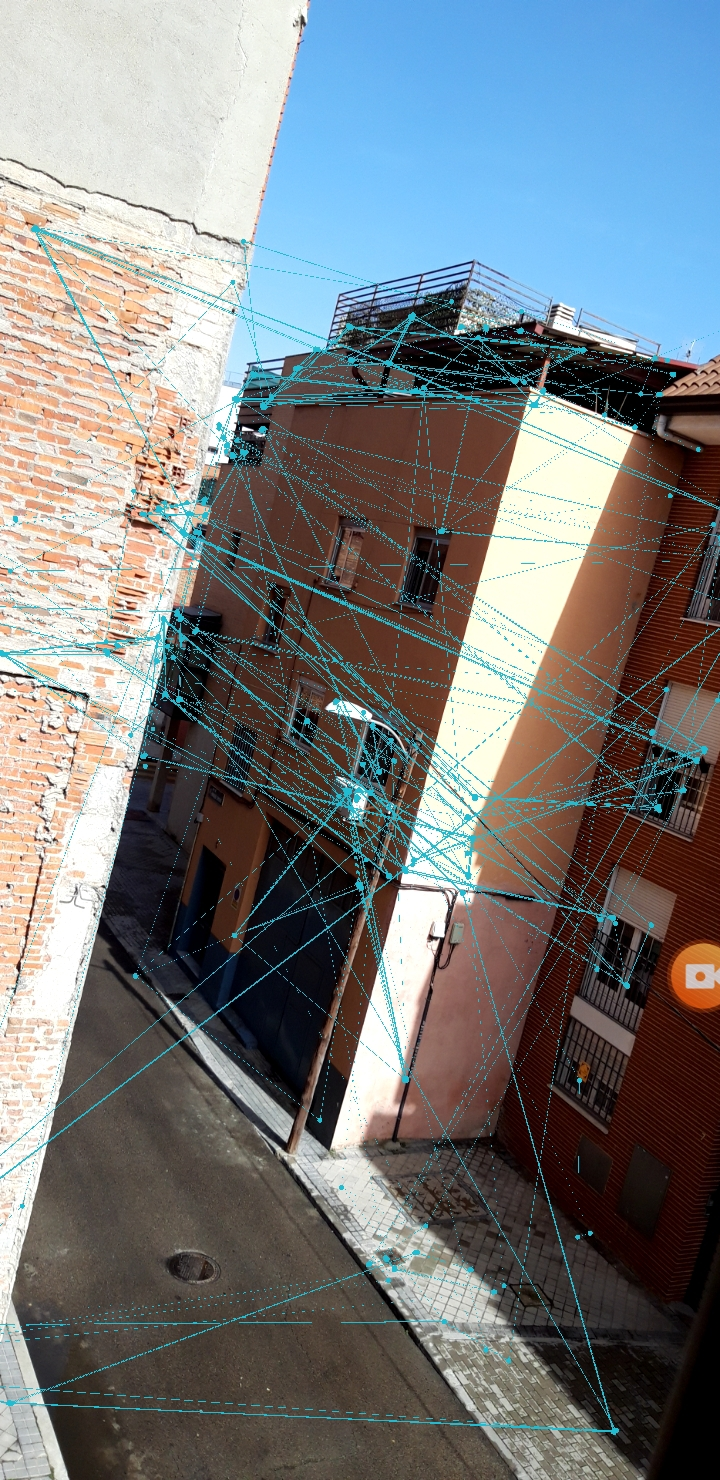
\includegraphics[scale=0.2]{Sections/Contribuciones/Imagenes/LineRenderer.jpg}
    \caption[Prueba de concepto para Line Renderer.]{Prueba de concepto para Line Renderer.}
    \label{fig:LineRender}
\end{figure}

Cuando ya estaban todos los puntos, la siguiente acción fue comprobar si existía verdaderamente una profundidad con estos.
En primer lugar, dentro del bucle principal de la aplicación, comprobaba la distancia máxima y mínima que un punto tenía con la cámara, y en base a eso a cada uno de los demás puntos les asignaba un gradiente de color, que en este caso iba de negro (más cercano a la cámara) a rojo. Sin embargo esto era demasiado costoso,
por lo que investigué el shader de profundidad explicado en el apartado \ref{sec:shaderProfundidad}. Tras modificar todos los parámetros del mismo disponibles, llegué a conseguir ver la distancia a la que los objetos se encontraban de la cámara.\\

\begin{figure}[H]
    \centering
    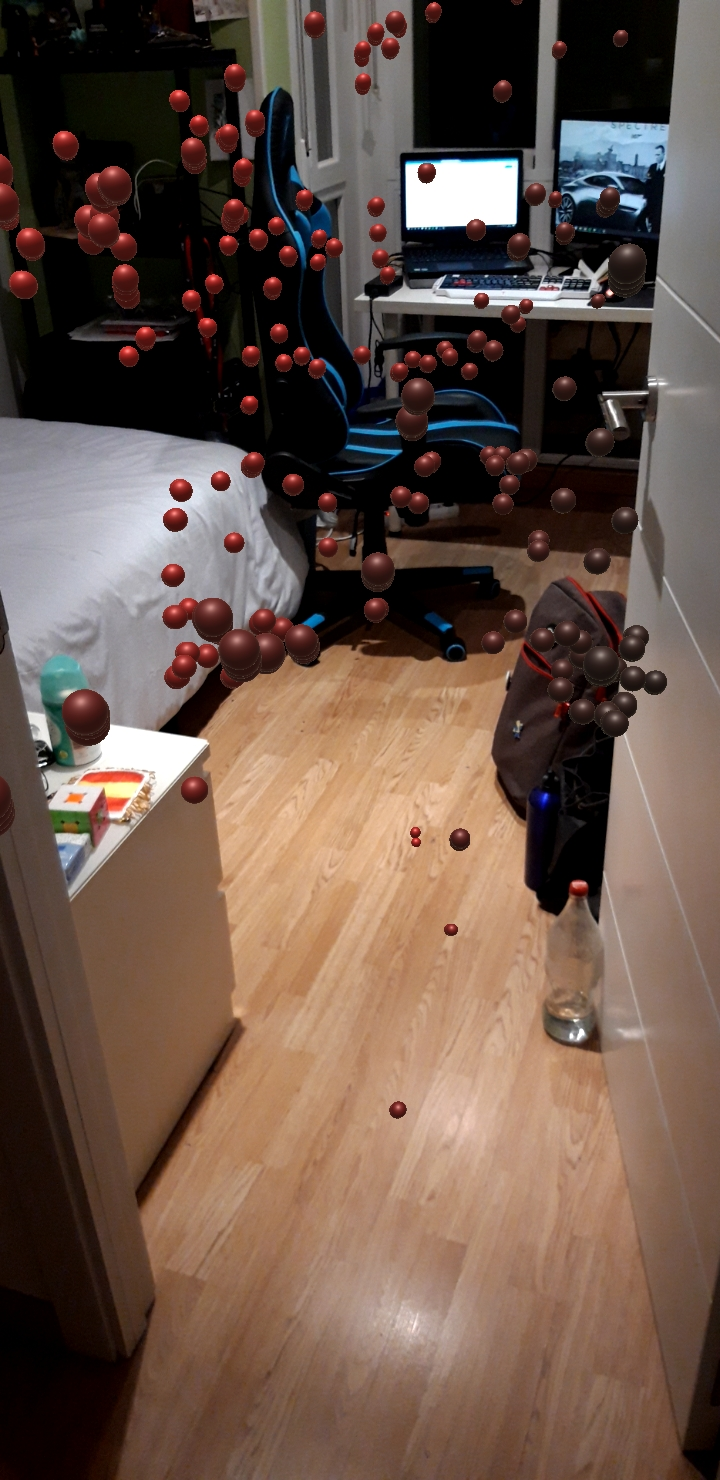
\includegraphics[scale=0.2]{Sections/Contribuciones/Imagenes/PuntosColores.jpg}
    \caption[Distancia de los puntos respecto a la cámara.]{Distancia de los puntos respecto a la cámara.}
    \label{fig:Puntos colores}
\end{figure}

Tras realizar esto, generé un proyecto común que contenía Mapbox y ARCore, pero debido a la imposibilidad de realizar pruebas por la situación excepcional del COVID-19, la aplicación se descartó y se continuó con las pruebas en aplicaciones individuales. 

En último lugar, creé la aplicación que genera todas las pruebas dentro de Unity así como la aplicación en Python que compara las imágenes de una serie de carpetas dadas y devuelve el resultado de estas comparaciones en archivos \textit{CSV}. La primera aplicación consistía en una ampliación de la que generaba la nube de puntos, incluyendo toda la información de rendimiento de la aplicación así como las funcionalidades de capturar la pantalla (desde la generación de la captura hasta el dónde y cómo se guarda la imagen resultante), activar y desactivar la nube de puntos, o todo el proceso de generar las pruebas mediante una corrutina y guardar los resultados. También añadí cierta prevención de errores por parte del usuario para hacerla un poco mas fácil e intuitiva.\\

En la aplicación de Python, partí de la base de \textit{OpenCV} para la comparación de imágenes y formé en base a ella una estructura que buscaba dada una única carpeta todas las subcarpetas y comparaba sus imágenes con un estado óptimo previamente creado. El resultado lo guarda como imagen en blanco y negro con sus diferencias en otra carpeta. Tras esto genera un archivo CSV por carpeta con el resultado de la comparación y uno final que comparaba todos estos archivos. Desde Photoshop, creé todas las imágenes de referencia uniendo las imágenes generadas por la aplicación.\\

Finalmente, realicé las pruebas con el dispositivo móvil para comprobar las diferencias de las nubes de puntos y poder anotar los resultados de ellas. Tanto las pruebas de oclusión como las de tiempo y la primera prueba de concepto. Por último realicé las pruebas que necesitaban de un ordenador portátil para conectar el dispositivo móvil.